\chapter{Grundlagen}
\label{sec:fundamentals}
\todo[color=blue!40]{Feedback zu Struktur des Literaturkapitels}\section{Software Qualitätssicherung}
\subsection{Motivation und Relevanz}

\todo{Evt. einleitende Worte...}
Der Funktionsumfang von Software stieg in den letzten fünzig Jahren enorm. Gleichzeitig bietet die Geschichte der Informatik viele Beispiele, die für die Notwendigkeit von Qualitätssicherung in der Softwareentwicklung sprechen. Ein sehr bildhaftes Beispiel der Folgen von fehlerhafter Software, ist die Selbstzerstörung der Ariane 5 Rakete im Jahr 1996 [QUELLE 1]\todo{Ref}. Das Trägheitsnavigationssystem wandelte eine 64-bit-Gleitkommazahl in eine Ganzzahl. Dieser Programmteil wurde schon in der Ariane 4 verwendet, nur war diese weitaus schubschwächer und der betroffene Sensor erzeugte viel kleinere Ergebnisse. Nur 36 Sekunden nach Start des Erstfluges, setzte also ein klassischer Überlauf ein und die Rakete aktivierte ihren Selbstzerstörungsmechanismus.
Ähnliches passierte bei der Raumsonde Mars Obiter der NASA. Diese war am 24. September 1999 gestartet und hätte 220 Millionen Kilometer später auf dem roten Planeten landen sollen. Kurz vor der Landung ging der Kontakt verloren, die Sonde zerschellte an der Oberfläche des Planeten. In diesem Fall war es kein Überlauf sondern ein Fehler bei den Maßeinheiten die den Steuerungsschub kontrollierten. Die Entwickler der NASA erwarteten in ihrem Code Zahlen in Form von Newton, während der Hersteller Lockheed Martin angloamerikanische Pfund lieferte.Durch Zufall fiel der Fehler während des gesamten Flugs nicht auf.[QUELLE 2 - 1]\todo{Ref} 
In keinem der beiden Vorfälle kamen Menschen zu Schaden, trotzdem waren die finanziellen Verluste enorm. Natürlich war die Komplexität dieser NASA-Projekte sehr hoch und wahrscheinlich nicht repräsentativ für Software die am Markt erhältlich ist, trotzdem wären beide Fehler durch Testing vermeidbar gewesen. Im Fall der Ariane 5 hätte es ausgereicht die Schnittstelle zum Steuercomputer mit Extremwerten zu testen. Man wäre schnell auf den Überlauf gestoßen und hätte die Umrechnung anpassen können. Auch Mars Orbiter hätte durch ausführliches Schnittstellen-Testing auf Basis von Verträgen, welche die beteiligten Software-Teams untereinander ausmachen, gerettet werden können.

\subsubsection{Der Zwang zu qualitativem Wachstum}
Die Qualität von Software erhöhte sich geschichtlich nicht im selben Maße wie ihre Funktionalität. Dafür werden von (Thaller)[QUELLE2 - 2]\todo{Ref} zwei Gründe genannt.

Der Drang nach Wachstum bei modernen Programmen negiert die Erfolge die Unternehmen durch erhöhte Anstrengungen in der Qualitätssicherung feiern könnten. Die Zahl der Fehler wird weitläufig gesenkt,  gleichzeitig nimmt der Funktionsumfang der Programme massiv zu. Dieser Umstand rührt daher, dass ständig neue Käuferschichten gewonnen werden müssen, die wiederum neue Features fordern.
Software dringt in Gebiete vor die von analoger Technik dominiert wurde. Aeronautik, Medizin und Finanzwesen verlangen nach großen Programmpaketen, die potenziell viele Fehlerquellen mit weichreichenden Folgen enthalten.

\subsubsection{Komplexe Systeme führen zu Fehlern}
Von der Programmierung in Hochsprachen bis zur Ausführung auf der Hardware müssen unzählige Schichten korrekt ineinander greifen um das gewünschte Ergebnis hervorzubringen. 
Daher sind

QUOTE „Komplexe Systeme analytisch in begrenzer Zeit nur unvollständig erfassbar. Fehler sind damit zwangsläufig die Folge“ [QUELLE3] \todo{Ref}

Gründe wieso Fehler auftreten sind mannigfaltig. Aus menschlicher Sicht können Fehler auf drei Ebenen auftreten [QUELLE 3]:\todo{Ref}


\paragraph{Kommunikation}
Jegliche Art von Kommunikation ist Transformation (vgl. SHANNON, 1976). Dabei passieren diese Transformationen nicht nur bei der Kommunikation zwischen zwei Menschen sondern auch bei der Transformation von Sprache in Verständnis. Naturgemäß bleibt bei diesen Transformationen Informationsgehalt verloren, abhängig von verschiedenen Rahmenbedingungen manchmal sogar sehr viel, beispielsweise wenn Information in einer Sprache übermittelt wird, welche nicht die Muttersprache von beiden Kommunikationspartnern ist.
Im technischen Umfeld gibt es darum viele Standardbegriffe, die möglichst genau definiert sind. So soll der Informationsverlust eingeschränkt werden.
Weiters spielt sich ein nicht unerheblicher Teil der Kommunikation auf unterbewusster Ebene ab.

\paragraph{Fachlichkeit}
Kunden oder Auftraggeber sind naturgemäß Experten auf ihrem Gebiet. Sie wollen Software um ihre fachlichen Ziele effektiver verfolgen zu können. Dem Software-Entwickler fehlt dieses Fachwissen. Dem Entwickler fehlt dieses Fachwissen oft.
Der Kunde hat sehr detaillierte Vorstellungen der Software, ihm fehlt aber die Fähigkeit auf technischer und fachlicher Ebene zu abstrahieren. Dies ist eine der Hauptaufgaben des Requirements-Engineer. Genau an dieser Stelle ist die Gefahr groß, dass durch fehlendes fachliches Wissen wichtige Zusammenhänge übersehen werden oder unwichtigen Details zu viel Aufmerksamkeit geschenkt wird.
Außerdem sind die technischen Möglichkeiten nur eingeschränkt für den Kunden fassbar. Gerade Aufwandsschätzungen sind für Entwickler schon schwierig Das hat zur Folge, dass die Entwickler oft Alternativen anbieten müssen welche möglicherweise nicht den exakten Anforderungen entsprechen.

\paragraph{Komplexität}
Die Komplexität der Problemstellung bestimmt über Machbarkeit und Fehlerpotenzial. Seit Anbeginn der Informatik wird versucht Komplexität auf ein überschaubares Maß herunterzubrechen. Sei es durch Zerlegung in möglichst kleine Aufgaben, visuelle Darstellungsformen oder Abstraktion zu bekannten Programmiermustern.
Komplexität wird dadurch aber niemals vermindert, sondern nur versteckt bzw. anschaulicher gemacht.


\subsection{Softwarequlität und Standards}
\subsection{Testprozess}
\subsection{Teststufen}
\subsubsection{Klassisches Vorgehen}
\subsubsection{Agiles Testen}
\subsection{Regressionstests und Testautomatisierung}
\subsection{Modellbasiertes Testen}
\subsubsection{Definition}
Im allgemeinsten Sinn, werden im modellbasierten Testing Testfälle aus Modellen abgeleitet, die das Sollverhalten eines Software-Systems beschreiben. (QUELLE BASISWISSEN MODELLBASIERTER SOFTWARETEST)\\

In (QUELLE PRACTICAL MODEL BASED TESTING) werden vier verschiedene Herangehensweisen zusammenfassend als modellbasiertes Testen definiert:

\begin{itemize}
\item Generierung von Testdaten aus einem Domänenmodell
\item Generierung von Testfällen aus einem Umgebungsmodell
\item Generierung von Testfällen aus einem Verhaltensmodell
\item Generierung von Test-Skripts aus einem abstrakten Test
\end{itemize}

Die Autoren legen den Schwerpunkt auf die generativen Aspekte. Weniger Aufmerksamkeit wird dem vorausgehenden Schritt geschenkt: Die Modellierung der genannten Modelle. (QUELLE BASISWISSEN MODELLBASIERTER SW TEST) nennt folgende  zentralen Merkmale des modelbasierten Testings:

\begin{itemize}
\item Die zu testende Software, ihre Umgebung oder der Test, wird über Modelle betrachtet.
\item Diese Modelle konzentrieren sich in abstrahierter Form auf besondere Eigenschaften des SUT (meist auf dessen Verhalten).
\item Diese Modelle können entweder eigenständig erstellt werden oder aus Entwicklungsmodellen abgeleitet werden.
\item Mit Testdaten und technologischen Adaptern kombiniert, bilden diese Modelle die Basis generierter Testfälle.
\end{itemize}

Dies führt zur pragmatischen Definition von modellbasiertem Testing:

\begin{quote}
Modellbasiertes Testen umfasst mindestens einen der beiden folgenden Aspekte: Tests modellieren oder Tests aus Modellen generieren.
\end{quote}

\subsubsection{Der MBT Prozess}
Model-based Testing automatisiert, einer nachvollziehbaren Strategie folgend \todo{Ref zu Pfadabdeckung usw}, die Erstellung der detaillierten Testfälle (Testscripts). \ref{utting}
\subsubsection{Modellkategorien}
Im Feld der modellgetriebenen Entwicklung und des modellbasierten Testens wird grundsätzlich zwischen drei verschiedenen Modellkategorien unterschieden.

\paragraph{Umgebungsmodelle} stellen den Ausschnitt der Domäne dar, wo das zu testende System platziert wird oder ist.
\paragraph{Systemmodelle} beschreiben das SUT in statischer und dynamischer Hinsicht. Sie stellen dar aus welchen Komponenten das SUT zusammengesetzt ist, welche Eigenschaften diese haben und wie diese miteinander kommunizieren. 
\paragraph{Testmodelle} dienen als Grundlage für die Generierung von Testfällen, basiernd auf Spezifikations- und Entwurfsdokumenten. Daher enthalten sie auch oftmals Teile von Umgebungs- und Systemmodellen. Weiters beschreiben sie den Ablauf der zu generierenden Testfälle. Möglich ist die Angabe darüber, welche Eingaben das SUT erhalten soll und welche Ausgaben bzw. Reaktionen erwartet werden.


\subsubsection{Vergleich mit klassischem Testing}

\subsection{Entscheidungshilfe für den Einsatz von MBT}
In der Praxis stellt sich für jedes Software-Projektteam die Frage welche Teststrategie am effizientesten, in Bezug auf Qualität und Ressourcennutzung ist. Manuelles Testen gilt in der Industrie immer noch als das am häufigsten eingesetzte Verfahren (QUELLE ARTIKEL STARTHILFE FÜR MODELLBASIERTES TESTEN), aber deren Wirksamkeit mindert sich mit steigender Komplexität der zu testenden Software. Skriptbasierte Testautomatisierungstools kommen seit Jahren in der Industrie zum Einsatz. Durch die automatisierte Testausführung, wird der Testprozess schnell und wiederholbar. Verglichen mit manuellen Tests sind skriptbasierte Tests zeitsparender und weniger fehleranfällig. Gleichzeitig müssen skriptbasierte Tests gewartet werden, was einen nicht unerheblichen Ressourcenaufwand bedeuten kann.\\
Als Alternative dazu steht das modellbasierte Testen. Basierend auf (QUELLE ARTIKEL STARTHILFE FÜR MODELLBASIERTES TESTEN) folgen acht Fragestellungen die zu einer Entscheidung bezüglich der Sinnhaftigkeit des Einsatzes von MBT führen sollen:

\todo{Grafik für Entscheidungshilfe (gerichteter Graph)}
\begin{itemize}
\item Wie komplex sind die Testbasis und die zu testende Funktionalität?
Die Komplexität des zu testenden Systems ist ein entscheidender Faktor, bei der Auswahl der passenden Teststrategie. Aus niedriger Komplexität oder allgemein wenig Funktionalität, resultieren wenig Testfälle, die mit manuellen Tests durchgeführt werden können. Diese erfordern wenig Planungsaufwand und können schnell ausgewertet werden. Bei steigendem Funktionsumfang kann eine skriptbasierte Ausführung der Testfälle sinnvoll sein. Außerdem kann modellbasiertes Testen die Generierung dieser Testfälle automatisieren.
\item Wie wichtig ist die Überdeckungsanalyse?
Im Software-Testing wird oft anhand der prozentualen Abdeckung des Quellcodes auf die Güte der Teststrategie geschlossen. Mittels skriptbasiertem Testen ist es aber nicht trivial festzustellen, welche Teile des Codes ein Testfall genau abdeckt. Mit MBT lässt sich anhand der Modellüberdeckung schneller feststellen welche Komponenten abgedeckt sind. Außerdem lassen sich Konzepte der Traceability (also der Verfolgbarkeit von Test zu Code) im MBT sehr einfach einführen. Modellbasierte Tests haben daher den nützlichen Nebeneffekt wie ein Vertrag, zwischen Requirement und tatsächlicher Funktionalität, zu funktionieren. Weil modellbasierte Tests oft einfach visuell dargestellt werden können, eignen sie sich auch zu Präsentationszwecken vor Kunden.
\item Wie häufig finden Änderungen in der Spezifikation statt? 
Unzufriedenheit mit skriptbasierten Tests entsteht oft aus teuren Wartungsarbeiten, die nötig werden sobald sich das zu testende System weiterentwickelt. Skriptbasierte Tests können nur zu einem gewissen Grad Änderungsunabhängig entwickelt werden. Gerade wenn das Softwareprojekt aus kurzen Entwicklungszyklen besteht (so wie es viele moderne agile Projekte sind), die viel Änderungspotenzial mit sich bringen, sollte MBT in Betracht gezogen werden.
\item Wie wichtig ist die Plattformunabhängigkeit der Testfälle?
Abhängig von der Testebene wo automatisierte Tests auf das System zugreifen, können skriptbasierte Tests nutzlos werden wenn beispielsweise der Austausch einer GUI-Bibliothek erfolgt. Da bei modellbasierten Tests eine strikte Trennung zwischen Testmodell und Adapter zum SUT gemacht wird, muss bei einem Plattformwechsel auch nur dieser Adapter angepasst werden. Auch bei industrieller Software die oft mittels dem Konzept der Software-Familien arbeitet, kann es von Vorteil sein wenn die eigentlichen Testkomponenten unabhängig von der Adapter-Logik bestehen.
\item Ist die Testbasis modellierbar?
Für die Modellierung des SUT ist eine Vielzahl von Notationen verfügbar. Zustandsbasierte und Ereignisbasierte \todo{Link zu einer Grundlagen section wo ich das erläutere} Notationsarten ermöglich die Modellierung sehr vieler funktionaler Eigenschaften. Wenn sich die Funktionalität der Testbasis aber nur unzureichend modellieren lässt, macht modellbasiertes Testen schlicht keinen Sinn.
\item Hat das Testteam Erfahrung mit Software-Modellierung? / Sind Modellierungskenntnisse im Testteam verfügbar?
Abhängig davon wie die Rollen im Projektteam verteilt sind, muss festgestellt werden ob Modellierungskenntnisse bei denjenigen vorhanden sind, die im weiteren Verlauf Testfälle erstellen und warten. Das Testteam muss deshalb möglicherweise geschult werden. Die Kosten dieser Schulungen, verglichen mit den Aufwänden für manuelles und skriptbasiertes Testen, können entscheidend für die Wahl von MBT sein.
\item Kann das Test-Orakel automatisiert werden?
Da beim modellbasierten Testen, Testfälle in der Regel automatisch generiert werden, sollen auch die erwarteten Testergebnisse modelliert oder in Form von Testdaten hinterlegbar und automatisch prüfbar sein. Falls die erwarteten Systemeigenschaften nicht modellierbar sein können, muss jeder Testfall manuell geprüft werden. Dieser Umstand mindert die Nützlichkeit von modellbasiertem Testen.
\item Ist die Bereitschaft für den Kauf und Einführung eines MBT-Werkzeugs vorhanden?
Eine Einführung von MBT ist immer auch mit Anschaffungskosten verbunden. Auf dem Markt sind verschiedenste Werkzeuge erhältlich \todo{Link zu Marktübersichts Section}. Weiters muss sich das gewählte Tool aber auch in bestehende Umgebungen integrieren lassen (was oft mit weiteren Kosten verbunden ist).
\end{itemize}

\subsubsection{Tool-Landschaft}
Wie auf dem Feld der skriptbasierten Testautomatisierung, ist die Auswahl an Tools zur Unterstützung von modellbasierten Tests vielfältig.Modellbasiertes Testen umfasst in der Regel mehrere Aktivitäten, für die jede Kombination aus passenden kommerziell erhältlichen Werkzeugen herangezogen werden können. Auch die marktführenden Tool-Hersteller haben begonnen ihre Testing Applikations-Suiten für MBT auszurüsten. 

\section{State of the Art - Modellbasiertes Testen}

State of the art
In diesem Kapitel wird ein Überblick über bereits existierende Lösungen für die Problemstellung bzw. verwandte Problemstellungen gegeben. Dabei ist eine Klassifizierung der existierenden Lösungen empfehlenswert. Eine Analyse der Lösungen, nach Kriterien sortiert, sollte insbesondere auch die Defizite der existierenden Lösungen erläutern und damit insbesondere auch eine Begründung liefern, warum diese Lösungen für die Problemstellung der Arbeit nicht herangezogen werden können.

Unterkapitel----------------------------------------------------------------------

Bei der Verwendung von Gliederungsebenen gibt es Folgendes zu beachten:
\begin{itemize}
	\item Es sollten nicht mehr als 3 Gliederungstiefen nummeriert werden.
	\item Unterkapitel sind nur dann sinnvoll, wenn es auch mehrere Untergliederungen gibt. Ein Kapitel 2.1.1 sollte somit nur dann verwendet werden, wenn es auch 2.1.2 gibt.
	\item Oft ist es einfacher und besser verständlich, Aufzählungen als Text zu formulieren und somit weitere Gliederungsstufen zu vermeiden.
\end{itemize}

Abbildungen
Beschreibungen zu Abbildungen und Tabellen stehen unter dem Bild. Jede Abbildung muss im Fließtext referenziert werden. In \LaTeX besitzen Abbildungen typischerweise Labels, welche zum referenzieren verwendet werden. Zudem plaziert \LaTeX die Abbildungen an geeigneten Stellen, was meistens auch wünschenswert ist. Falls das nicht gewünscht wird, kann es durch Optionen beeinflusst werden.

Abbildung \ref{fig:xxx} verdeutlicht  \dots\\
(siehe Abbildung \verb|\ref{<label>}|)

\begin{figure}
	\centering
	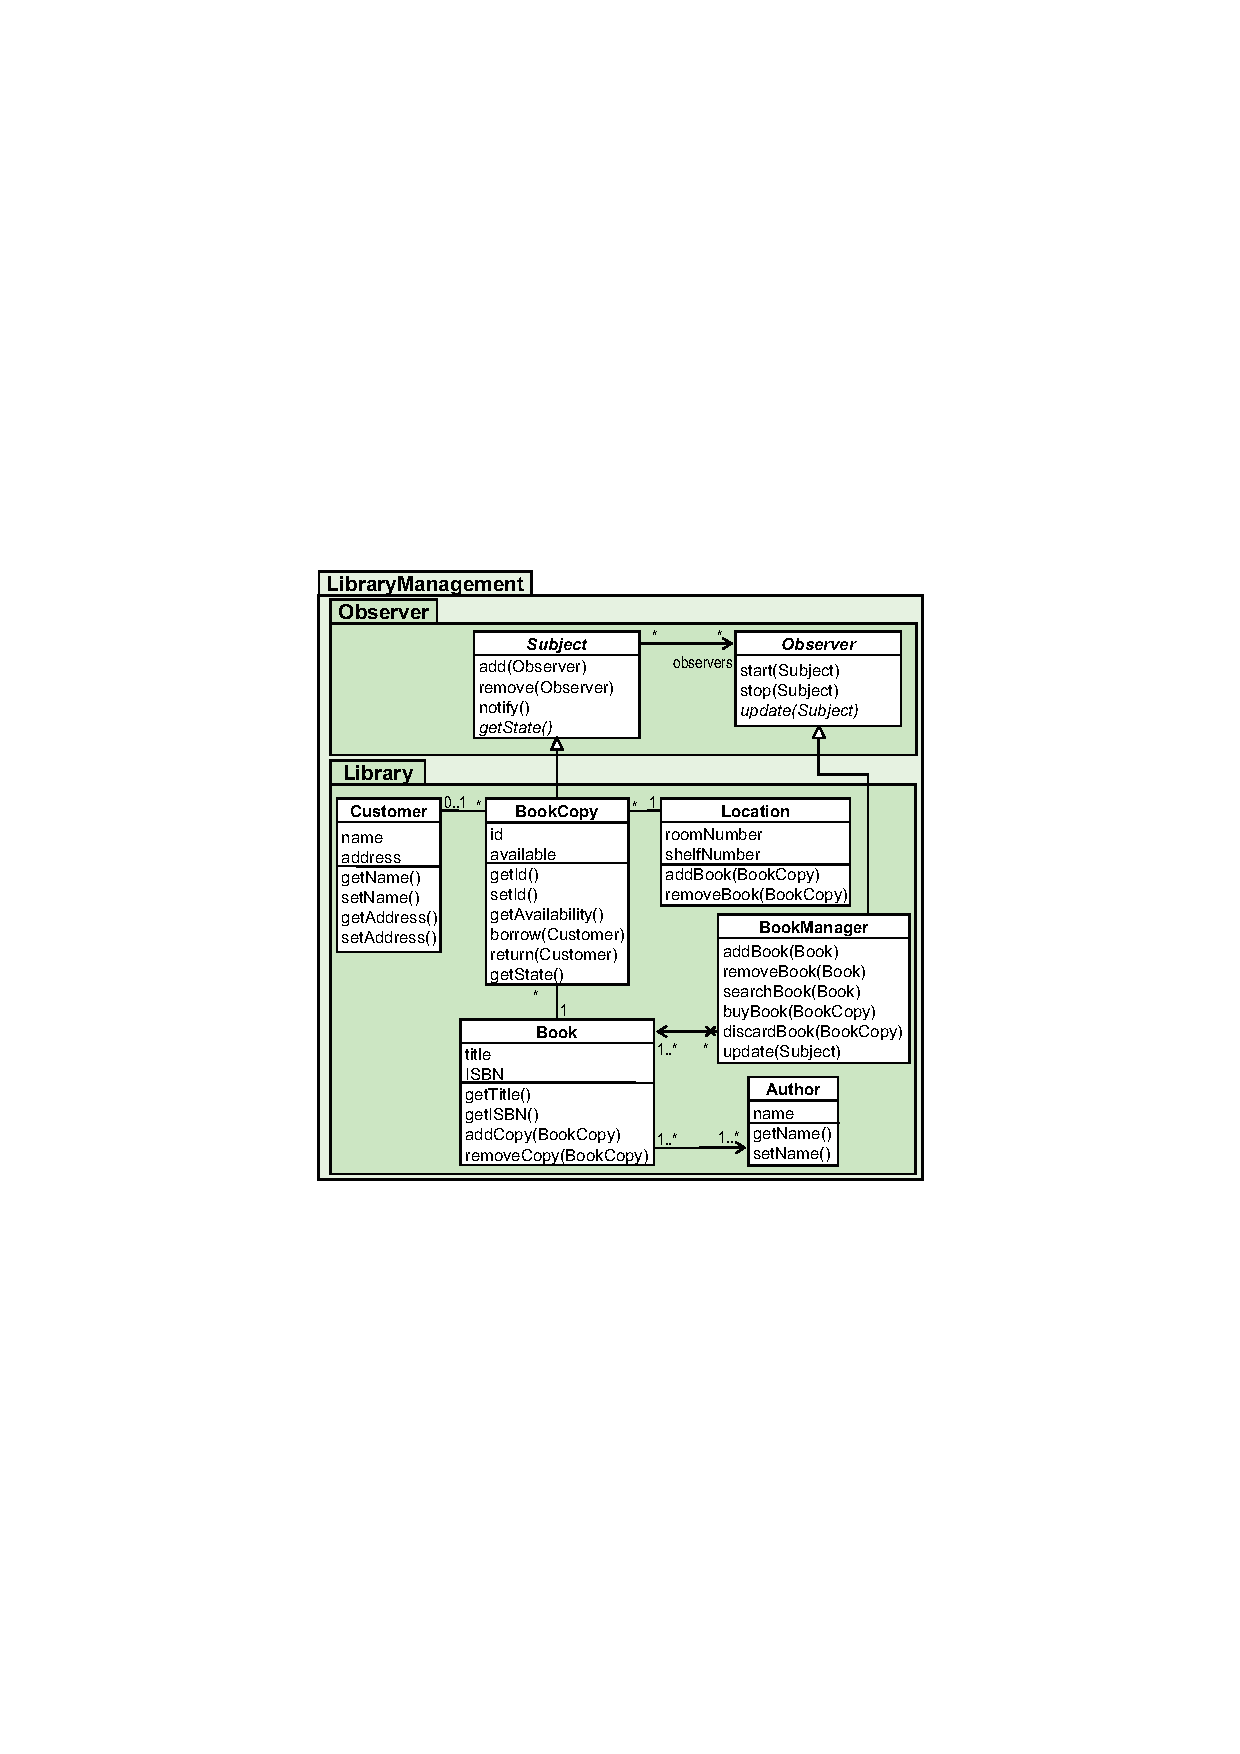
\includegraphics[width=0.4\linewidth]{figures/figure1}
	\caption{xxx (Quelle zitieren, wenn nicht selbst erstellt)}
	\label{fig:xxx}
\end{figure}
Tabellen
Jede Tabelle muss im Fließtext referenziertw werden. Für Tabellen gelten die selben Regeln, wie für Abbildungen (siehe dazu Abschnitt \ref{sec:abbildungen}).

Eine Beispiel einer Tabelle ist in Tabelle \ref{tab:xxx} zu finden:
\begin{table}
	\centering
	\begin{tabular}{| >{\bfseries}l | c | r | }
		\hline
			\rowcolor{orange} \bfseries Linksbündig & \bfseries Zentriert & \bfseries Rechtsbündig \\
		\hline
		\hline
			Zeile 1 & xxx & xxx \\\hline
			Zeile 2 & xxx & \dots \\\hline
			\multirow{2}{*}{Zeile3}
			& xxx & xxx \\\cline{2-3}
			& xxx & xxx \\\hline
		\hline
			\multicolumn{3}{| c |}{xxx} \\\hline
	\end{tabular}
	\caption{xxx (Quelle angeben)}
	\label{tab:xxx}
\end{table}

Bitte beachten Sie, dass Tabellen generell so einfach wie möglich gehalten werden sollen. Tabelle \ref{tab:xxx} dient unter anderem dazu Studierenden zu zeigen, wie Tabellen in \LaTeX\xspace erstellt werden können und wie Farben verwendet werden.